\subsection{INDEPENDENT SET}
\textbf{Given:} Graph G = (V,E), target K. \\
\textbf{Question:} Does there exist $I \subseteq V$ such that $|I| \geq K$\\ and for all $u,v\in I$ we have $(u,v) \notin E$? 
\subsection{CLIQUE}
\textbf{Given:} Graph G = (V,E), target K. \\
\textbf{Question:} Does there exist $C \subseteq V$ such that $|C| \geq K$\\ and for all $u,v\in C$ we have $(u,v) \in E$?
\subsection{VERTEX COVER}
\textbf{Given:} Graph G = (V,E), budget B. \\
\textbf{Question:} Does there exist $C \subseteq V$ such that $|C| \leq B$\\
and for all $(u,v) \in E$ we have $(u \in C \lor v \in C)$?
\subsection{MAX CUT}
\textbf{Given:} Graph G = (V,E), target K. \\
\textbf{Question:} Does there exist a cut  $(S,V\setminus S)$ of size at least K?\\
\subsection{MAX BISECTION}
\textbf{Given:} Graph G = (V,E), target K.\\
\textbf{Question:} Does there exist a cut  $(S,V\setminus S)$ of size at least K, such that $|S| =  |V \setminus S|$?
\subsection{BISECTION WIDTH}
\textbf{Given:} Graph G = (V,E), target K.\\
\textbf{Question:} Does there exist a cut  $(S,V\setminus S)$ of size at most K, such that $|S| =  |V \setminus S|$?
\subsection{HAMILTONIAN PATH}
\textbf{Given:} Graph G = (V,E).\\
\textbf{Question:} Does G have a path that visits every vertex exactly once?\\
\subsection{TSP}
\textbf{Given:} Distance matrix D, target t. \\
\textbf{Question:} Is there a tour of length at most t that visits every node in the graph defined by D exactly once?\\
\subsection{SET COVERING}
\textbf{Given:} 
A set U(universe). A collection of subsets $S_1,S_2,...,S_n \subseteq U$\\
\textbf{Question:} Does there exist B subsets whose union is U?
\subsection{EXACT COVER BY 3-SETS}
\textbf{Given:} 
A set U of size 3m. A collection of subsets $S_1,S_2,...,S_n \subseteq U$ of size three.\\
\textbf{Question:} Does there exist m subsets which cover U exactly? 
\subsection{TRIPARTITE MATCHING}
\textbf{Given:} 
Three sets B, G, H of size n. A collection of triples $T \subseteq B \bigtimes G \bigtimes H.$\\
\textbf{Question:} Does there exist n triples such that every element of B, G and H is contained in exactly one of these triples?
\subsection{SET PACKING}
\textbf{Given:} 
A set U. A collection of subsets $S_1,S_2,...,S_n \subseteq U$. A goal K.\\
\textbf{Question:} Does there exist k pairwise disjoint subsets?
\subsection{KNAPSACK}
\textbf{Given:} 
N items. Item i has value $v_i$ and weight $w_i$, both positive integers. A max weight W. And a goal K. \\
\textbf{Question:} is there a subset of the N items such that the total weight is at most W and that the total value is at least K?
\subsection{SUBSET SUM (SPECIAL CASE OF KNAPSACK)}
In this version of knapsack an items value is equal to its weight, and the goal K is equal to the max weight W. So, we are given a set of N integers and an integer K and ask if there is a subset of the given integers that adds up to K.
\subsection{BIN PACKING}
\textbf{Given:} 
N positive integers and two more integers C(capacity) and B(number of bins).  \\
\textbf{Question:} can these numbers be partitioned into B subsets, each of which has a total sum of at most C?
\subsection{NAESAT $\le$ MAX CUT}
\textbf{Theorem 9.5:} MAX CUT is NP-Complete\\\\
We prove this by reducing from NAESAT, which we know is NP-complete.\\\\
We construct a graph G = (V,E), and a goal K such that there is a way to separate the nodes og G in to two sets S and V-S with K or more edges  going from one set to the other, if and only if there is a truth assignment for our NAESAT formula f which satisfies f. We allow more than one edge between two vertices, and each such edge contributes one to the cut. 
\\\\
Our input formula has m clauses and n variables, and we constuct a graph with 2n nodes - one for each variable and it's negation. For each clause, we add edges to our graph to form triangles. If two literals of a clause are the same, for example $(x \lor y \lor y)$, (which is equivalent to $(x \lor y)$), we just add two edges between the nodes representing the two destinct literals. The point of the triangles and the two edges between same literals, is that for both constructs, the cut is always two. Now we add an edge between variables and their negation, and set our target K = n + 2m. \textbf{The n is for cutting the horizontal edges, and 2m is because we need to cut each triangle (each clause) - if we don't, then it is possible for all literals in a single clause to be true (and then it's not naesat))}. This completes the reduction.\\\\
\textbf{Example:}\\
Given a NAESAT formula:  $f =  (x_1 \lor x_2) \land (x_1 \lor \lnot x_3) \land (\lnot x_1 \lor \lnot x_2 \lor x_3)$\\
We can construct the graph shown in figure 4. The green edges come from the first clause, red the second clause, and blue the third clause.\\
\begin{center}
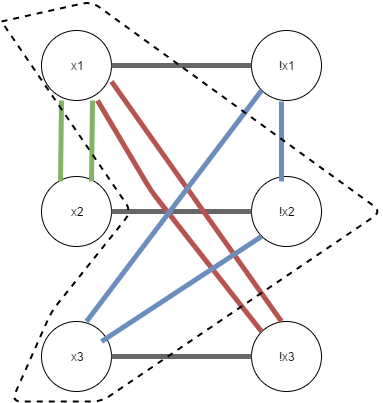
\includegraphics[scale=0.5]{NAESATtoMAXCUT}\\
\textbf{Figure 4:} Graph r(f) corresponding to the formula f
\end{center}
\textbf{Analysis:}\\
For each variable we add two nodes and one edge between them. For each clause we add at most 3 edges. So the reduction is polynomial.\\\\
$\implies$ :\\
Given a satisfying naesat assignment for f, we must show that r(f) has a cut of size at least K. $x_1 = 1, x_2 = 0, x_3 = 1$ is a satisfying assignment for f. We have 3 variables and 3 clauses, so the target K is $2*3+3 = 9$. The cut of 9 is obtained by cutting the vertices within the dotted line in the example above. 
\\\\
$\impliedby$ :\\
Given a cut of size at least K of r(f), we must show that there is a satisfying naesat assignment for x. Here we just take the truth values of the nodes in our cut set.
\\\\\\
\textit{Read more in papadimitriou page 191-192.}
\newpage

